\chapter{Idémyldring}
I dette steget i prosessen er målet å generere en liste over det vi tror kan være mulige årsaker til problemet. Det er en del forskjellige verktøy en kan bruke for å oppnå dette, men vi har valgt å benytte Idémyldring på bakgrunn av verktøyets egenskap til å generere mange idéer hurtig.

\section{Idémyldring}
I rotårsaksanalyse finnes det to ulike måter å gjennomføre Idémyldring på, Strukturert- og Ustrukturert Idémyldring. I den strukturerte versjonen får hver deltaker sin tur til å komme med en idé, og dette sikrer at alle får delta like mye. På den ustrukturerte måten kan alle komme med idéer når de dukker opp, og fungerer mye mer spontant enn den strukturelle. Det er spesielt viktig å ikke omformulere eller diskutere forslagene etterhvert som de kommer, dette skal gjøres etter Idémyldringsøkten er over.

\subsection{Ønsket utbytte}
Ønsket utbytte i denne delen er en mengde idéer som kan legges til grunn når det utføres statistisk arbeid på rotårsakene. Det er spesielt ønskelig å kunne ende opp å utvikle spørsmål til brukerundersøkelser basert på noen av disse årsakene.

\subsection{Gjennomførelse}
Det første som ble gjort når økten startet var å kommunisere og skrive opp problemstillingen på en tavle. Vi valgte å strukturere Idémyldringen som et tankekart ettersom dette var en kjent løsning for gruppen, og brukte den ustrukturerte tilnærmingen til Idémyldringen på grunn av dens uformelle og spontane natur. 

Det første problemet vi så på var hvorfor personer bruker Torrents til å laste ned opphavsrettsbeskyttet materiale. Når idéstrømmen begynte å gå langsomt, stoppet vi og vurderte det vi hadde kommet fram til. Vi kom blant annet fram til at vi burde spesifisere problemstillingen ytterligere og valgte derfor å spesifisere den til hvorfor folk laster ned på skolenettet. Vi forkortet dette til: ``Hvorfor Torrenting på skolenettet'' for enkelthets skyld. Det ble kjørt enda en økt med denne nye problemstillingen og fikk mer spesifikke resultater. 

\subsection{Resultater}
Etter øktene var ferdig ble det gjort en vurdering av resultatene og de ble kategorisert i henhold til likhetstrekk, under en fellesnevner som for eksempel Økonomi. Resultater og gruppering er som vist i \hyperref[fig:idemyldring]{Figur 4} under.

\begin{figure}[H]
    \centering    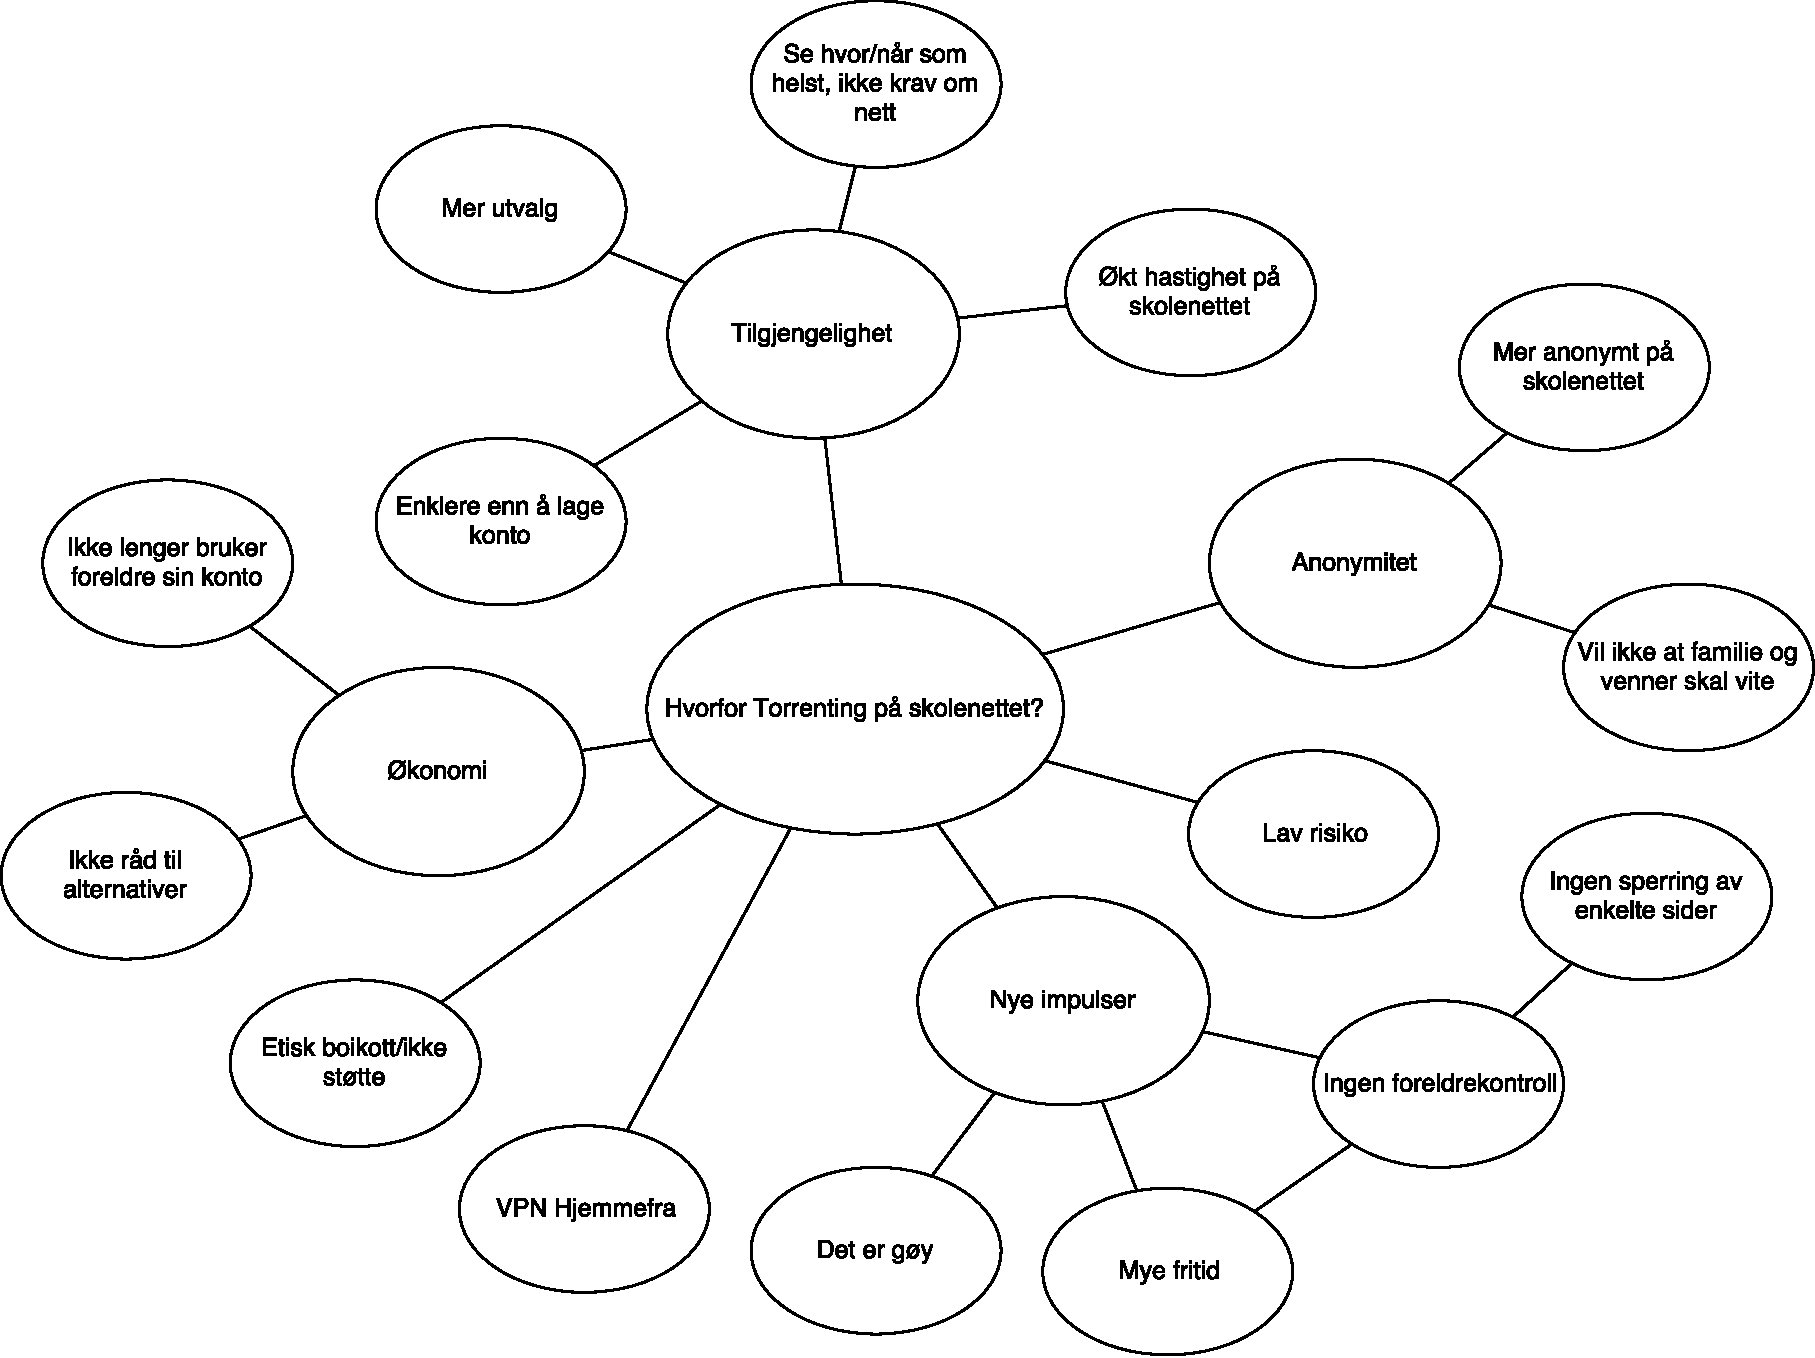
\includegraphics[scale=0.45]{case_1/bilder/idemyldring}
    \label{fig:idemyldring}
    \caption[Idémyldring]{Resultater og gruppering av idémyldringen}
\end{figure}

Resultatene er gruppert inn i fire hovedkategorier, Økonomi (som går på kjøpekraften til den enkelte person), Tilgjengelighet, Anonymitet (I forhold til at foreldre kan overvåke kjøp på nett, og at på skolenettet er du én blant mange), og tilslutt nye impulser i form av mer frihet og fritid, og påvirkning av kulturen.

Merk at noen årsaker kunne ikke plasseres i én kategori og er derfor direkte knyttet til problemstillingen. 


\subsection{Konklusjon av verktøyet}
Dette var en effektiv metode for å få en overordnet oversikt av hva årsakene kan være til at noen velger å laste ned opphavsrettsbeskyttet materiale, spesielt på skolenettet. Verktøyet fungerte bra i denne sammenhengen fordi gruppen hadde en del basiskunnskap om temaet fra før. Vi antar at en slik metode vil fungere dårligere dersom problemet ikke er forstått godt nok og/eller det er lite kunnskap om problemstillingen på forhånd.